\chapter{Resultados}
\label{chap:resultados}

% TODO Inlcuir datos de las máquinas

\section{TFHE}

\subsection{Tiempos de ejecución}

Al ser una ejecución ``especulativa'', la optimización de las funciones está muy limitada (se tiene que operar con todos los bits, gestionando el flujo de los datos eligiendo los valores con los que se opera mediante la puerta \verb|MUX|). Sin embargo, siempre que el circuito lógico sea cerrado para un número concreto de bits (de forma similar a un circuito físico), pueden utilizarse métodos formales y algebraicos para aumentar su eficiencia.

Por otro lado, crear algoritmos que sean versátiles con respecto al número de bits hace que estos circuitos lógicos tengan que hacer operaciones redundantes, o introducir demasiada complejidad ciclomática para estar preparado para cualquier tamaño de palabra.

\subsubsection{Operaciones aritméticas}

Según la documentación de TFHE, cada puerta lógica tarda 13ms en ejecutarse, y las puertas MUX tardan 26ms. Sabiendo que sólo el $ 13\% $ de las puertas lógicas en nuestro código son puertas MUX podemos establecer un tiempo por puerta de unos 15ms para calcular el tiempo teórico que deberían tardar nuestras operaciones en función del número de puertas lógicas que emplean. En la tabla \ref{table:time_by_gates} podemos ver los resultados del cálculo.

\begin{table}[]
    \centering
    \begin{tabular}{r | cc}
        operación       & puertas logicas       & tiempo estimado \\
        \hline \hline
        compare\_bit     & 2     & 0,04 \\
        equal   & 128   & 2,56 \\
        is\_negative     & 1     & 0,02 \\
        minimum/maximum & 388   & 7,76 \\
        add\_bit & 5     & 0,1 \\
        sum     & 320   & 6,4 \\
        negativo        & 192   & 3,84 \\
        resta   & 512   & 10,24 \\
        multiply        & 46826 & 936,52 \\
        mayor\_igual     & 128   & 2,56 \\
        shiftl/shiftr   & 771   & 15,42 \\
        u\_shiftl/u\_shiftr       & 129   & 2,58 \\
        divide  & 85776 & 1715,52 \\
    \end{tabular}
    \caption{Tiempo estimado de ejecución}
    \label{table:time_by_gates}
\end{table}

Hemos medido los tiempos de ejecución de las distintas operaciones aritméticas con varios tamaños de palabra (de 4, 8, 16, 32 y 64 bits). En la figura \ref{fig:crec_func} podemos observar como prácticamente todas tienen un crecimiento lineal con mayor o menor pendiente: hay algunas que son casi gratuitas, como las operaciones \verb|shift|; y hay otras como la resta, que crecen un poco más rápido (porque están compuestas por varias operaciones crecientes) pero sin perder su comportamiento lineal.

\begin{figure}[h]
    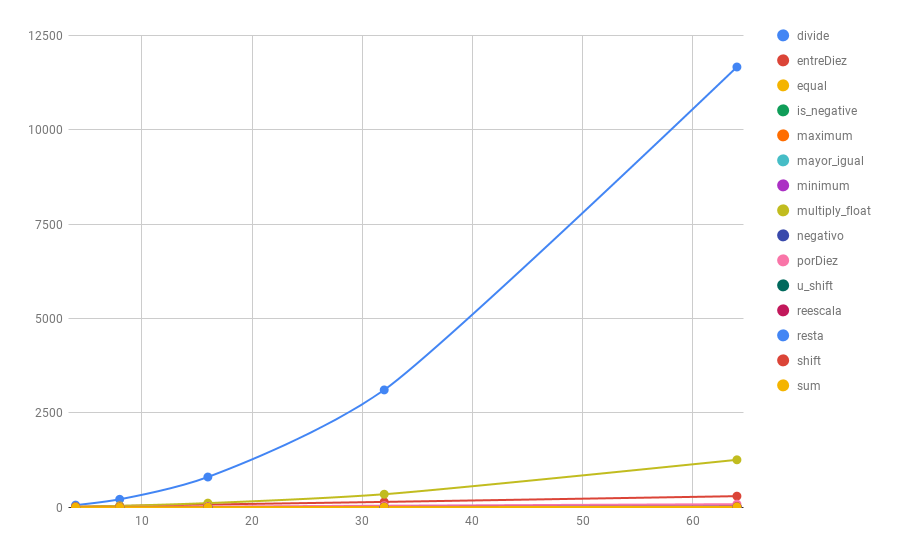
\includegraphics[width=\textwidth]{crec_func}
    \caption{Tiempo de ejecución por número de bits}
    \label{fig:crec_func}
\end{figure}

Sin embargo hay dos operaciones que crecen de una forma más preocupante: la multiplicación y la división. En ambas funciones se juntan tres factores:

\begin{enumerate}
    \item Requiere el uso de un gran número de funciones adicionales: sumas, restas, comparaciones, etc; haciendo que crezca el número de puertas lógicas.
    \item Debido a su complejidad, tiene varios bucles anidados cuyas iteraciones están relacionadas con el número de bits.
    \item Abordamos las operaciones trabajando con el doble de bits de la entrada. Es decir, un número de 64 bits se opera como si tuviese 128 para evitar desbordamientos.
\end{enumerate}

En la tabla \ref{table:ops_real_time} vemos cuáles son estos tiempos con números de 64 bits.

\begin{table}[]
    \centering
    \begin{tabular}{cc}
        Operación       & Tiempo (s) \\
        \hline \hline
        compare\_bit     & 0 \\
        is\_negative     & 0 \\
        u\_shift       & 0 \\
        add\_bit & 0 \\
        equal   & 3 \\
        mayor\_igual     & 4 \\
        min / max & 14 \\
        sum     & 8 \\
        negativo        & 8 \\
        resta   & 16 \\
        shift   & 19 \\
        multiply        & 1257 \\
        divide  & 11662
    \end{tabular}
    \caption{Tiempo real de ejecución}
    \label{table:ops_real_time}
\end{table}

En la figura \ref{fig:crec_div_mult} se puede ver cómo el crecimiento de cada valor con respecto al anterior  ($f(2^x)/f(2^{x-1})$ con $x$ número de bits) de ambas funciones corresponde con un crecimiento potencial con respecto al número de bits.

\begin{figure}[h]
    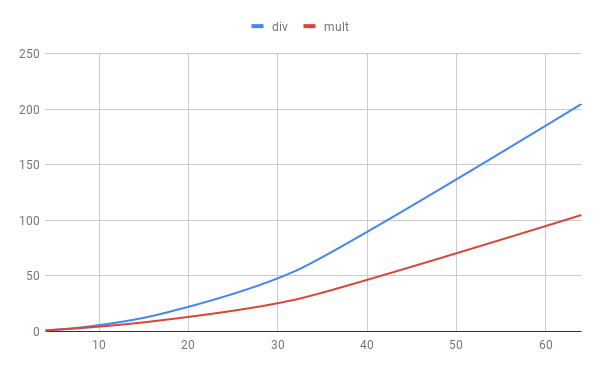
\includegraphics[width=\textwidth]{crec_div_mult}
    \caption{Crecimiento: división y multiplicación}
    \label{fig:crec_div_mult}
\end{figure}
% ---

Por último, calcularemos el tiempo teórico que tardarían en realizarse las operaciones de la curva de regresión (sumando los tiempos de sus sumas, multiplicaciones, divisiones...) y lo compararemos con el tiempo que han tardado realmente.

En la tabla \ref{table:sub_ops_r2} analizamos las operaciones contenidas en cada uno de los cálculos (ver anexo \ref{appendix:regresion_cuadratica}) y el tiempo estimado que tardarían en función de los tiempos mostrados en la tabla \ref{table:ops_real_time} .

\begin{table}[]
    \centering
    \begin{tabular}{r | c c c c}
        Cálculo & Sumas & Multiplicaciones  & Divisiones  & Tiempo  estimado (s) \\
        \hline \hline
        initVectores  & 7 & 5 & 0 & 76092 \\
        calcCuadrados & 0 & 4 & 0 & 5028 \\
        calcDuplas  & 0 & 9 & 0 & 11313 \\
        calcComplejos & 0 & 10  & 0 & 12570 \\
        CalcC & 6 & 0 & 4 & 46776 \\
        CalcB & 4 & 2 & 1 & 14208 \\
        CalcA & 2 & 2 & 1 & 14192 \\
        Total & 9 & 32  & 6 & 180179 \\
    \end{tabular}
    \caption{Sub-operaciones de regresión cuadrática}
    \label{table:sub_ops_r2}
\end{table}

En la tabla \ref{table:t_r2} vemos el tiempo total que han tardado en realizarse estas operaciones frente al calculado.

\begin{table}[]
    \centering
    \begin{tabular}{r | c c c c}
        Cálculo & Tiempo estimado (s) & Tiempo real (s) & Proporción \\
        \hline \hline
        initVectores  & 76092 & 235885  & 3,09 \\
        calcCuadrados & 5028  & 15687 & 3,11 \\
        calcDuplas  & 11313 & 35608 & 3,14 \\
        calcComplejos & 12570 & 75325 & 5,99 \\
        CalcC & 46776 & 220161  & 4,70 \\
        CalcB & 14208 & 264239  & 18,59 \\
        CalcA & 14192 & 352023  & 24,80 \\
        Total & 180179  & 1198928 & 6,65 \\
    \end{tabular}
    \caption{Tiempo real de regresión}
    \label{table:t_r2}
\end{table}

Se puede apreciar que hay referencias con respecto a los datos teóricos. Pueden deberse a que no sólo se está ejecutando el programa, si no la propia lógica que ejecuta el programa, pequeñas diferencias de tiempo en la ejecución de las puertas lógicas, o incluso puertas lógicas que hayamos obviado (como las de inicialización) que acumuladas puedan ser significativas.

\subsection{Límites de cómputo}

No los hay, más allá de los relacionados con la codificación al devolver el resultado plano, pero hay que estar pendiente (muy pendiente) del crecimiento cuando se opera, y a medida que aumenta el tamaño de los datos, aumenta notablemente el tiempo de ejecución.

Por ejemplo, para determinar cuántos bits necesitábamos para nuestra regresión cuadrática calculamos con $X$ el mayor valor de las $x$ (en nuestro caso 12), $n$ el mayor grado alcanzable (el mayor número de multiplicaciones que se podían acumular sobre ese valor), $d$ el número de bits para decimales y añadiéndole 1 (el bit del signo):

\begin{gather}
bits\_necesarios = n * (\log_2{X}) + d + 1 = 51
\end{gather}

Podríamos haber implementado la solución con números de 51 bits sin problemas, pero decidimos hacerlo con 64 para poder contrastar los resultados con los obtenidos evaluando las operaciones de forma individual.

\subsection{Problemas encontrados}

A medida que hemos ido desarrollando la solución hemos encontrado principalmente problemas derivados de tener que trabajar con número en un sistema de puertas lógicas: implementar los algoritmos, gestionar el signo, los decimales, etc; sin tener casi documentación ni librerías de apoyo. Es decir, uno de los principales problemas de TFHE es que cualquier solución se tiene que construir desde la base, como si efectivamente se estuviese programando en ensamblador y sin poder acudir a librerías de código abierto o documentación de ningún tipo (mas allá de la propia del sistema).

Aunque este es un problema importante a la hora de realizar una implementación destinada al uso comercial, desde el punto de vista del tiempo de implantación (hay que invertir muchas horas), es principalmente un problema para la estabilidad de las soluciones, que se basan en sistemas que no han sido probados previamente por nadie (se ha invertido casi el mismo tiempo en desarrollar nuestra solución que en depurarla y arreglar errores).

Pero sin lugar a dudas el mayor problema es el de la eficiencia: si bien nuestra solución es optimizable, el cálculo de una curva de regresión con la maqueta en \textit{python} (ver \ref{appendix:regresion_cuadratica}) tarda menos de $50$ ms, frente a las $50,88$ segundos ($2,1$ días) del cálculo cifrado.

\section{SEAL}

\subsection{Tiempos de ejecución}

Hemos probado los tiempos de ejecución con las siguiente operaciones.

\begin{itemize}
    \item Codificación de variable
    \item Codificación de variable como matriz
    \item Cifrado
    \item Cifrado de matriz
    \item Multiplicación
    \item Suma
\end{itemize}

En todas ellas, y con números de 8192, 16384 y 32768 bits, la ejecución se realiza de forma prácticamente instantánea (menos de un segundo). En el apéndice \ref{appendix:benchmarks_seal} se pueden ver los resultados en bruto de la ejecución de los tests incluidos en la documentación de SEAL. En la tabla \ref{table:benchmarks_seal} podemos ver un resumen.

\begin{table}[]
    \centering
    \begin{tabular}{r | c c}
        Operación   & BFV & CKKS  \\
        \hline \hline
        encode  & 410  & 12753 \\
        decode  & 359  & 34802 \\
        encrypt & 15324 & 20628 \\
        decrypt & 7145  & 1055 \\
        add & 344 & 300 \\
        multiply  & 76506  & 3567 \\
        multiply plain  & 12462  & 1140 \\
        square  & 54013  & 2662 \\
        relinearize & 31034 & 33513 \\
        rotate vector  & 31823  & 36967 \\
        rotate columns  & 31432  & - \\
        rescale  & - & 11607
    \end{tabular}
    \caption{Tests de eficiencia de SEAL (microsegundos)}
    \label{table:benchmarks_seal}
\end{table}

\subsection{Límites de cómputo}

Para cada uno de los esquemas veremos un límite de cómputo distinto, dependiendo de qué parámetro determina la capacidad de operación:

\begin{itemize}
    \item El parámetro \verb|noise_budget| en el esquema BFV
    \item Los elementos dentro de la cadena de CKKS
\end{itemize}

Además cuando hablamos de límites no hablamos sólo del número de operaciones, sino que debemos incluir que en SEAL sólo podremos trabajar con números, y en resumen con sólo tres tipos de operación: suma, resta y multiplicación.

\subsubsection{BFV}

Con BFV la limitación de trabajar con números se amplía: sólo podemos trabajar con números enteros. El parámetro que determina cuántos cálculos se pueden hacer es \verb|noise_budget|. Como comentamos en el capítulo \ref{chap:teoria}, este parámetro se va reduciendo a medida que se opera, y si llega a 0 el número se vuelve irrecuperable.

Hemos evaluado estos límites mediante un programa que multiplica mientras el nivel sea mayor que cero. Probando con distintos tamaños (\verb|poly_modulus_degree|) bajo los parámetros recomendados por SEAL, obtenemos los resultados de la tabla \ref{table:seal_bfv_mult_depth}.

\begin{table}[]
    \centering
    \begin{tabular}{c c}
        \textit{poly\_modulus\_degree}   & Multiplicaciones realizables  \\
        \hline \hline \\
        $2^{13}$  & 1 \\
        $2^{14}$  & 4 \\
        $2^{15}$  & 9
    \end{tabular}
    \caption{Profundidad computacional máxima BFV}
    \label{table:seal_bfv_mult_depth}
\end{table}

Vemos que el número de productos realizable es similar al que podemos realizar con 64 bits en TFHE, pero es mucho más bajo realmente. Mientras que en nuestro ejemplo de TFHE podíamos realizar 10 productos sin ningún problema, en este sólo podemos realizar 8 (si nuestro test nos ha devuelto 9 significa que con 9 el resultado está corrupto), sólo con número enteros de hasta 60 bits.

\subsubsection{CKKS}

Con CKKS, por tamaño de la cadena. El primer y el último número de la cadena tienen que ser mayores que el número a cifrar/descifrar, y la suma de estos dos con los intermedios tiene que ser menos que  \verb|max coeff_modulus| bit-length. Para calcular el tamaño de la cadena seguiremos el siguiente procedimiento:

\begin{enumerate}
    \item Reservaremos 120 bits: 60 para el primer número de la cadena (el número que determinará la precisión del descifrado) y otros 60 para el último (que tiene que tener al menos el mismo número de bits que el más grande del resto de la cadena)
    \item Rellenamos los espacios intermedios con números de 40 bits mientras la suma de toda la cadena sea menor que el número máximo de bits asignable a \verb|coeff_modulus| (ver \ref{table:poly_vs_coeff_modulus}).
\end{enumerate}

Tras realizar este cálculo, obtendremos el tamaño de la cadena equivalente al número de multiplicaciones realizables de la tabla \ref{table:seal_ckks_mult_depth}.

\begin{table}[]
    \centering
    \begin{tabular}{c c }
        \textit{poly\_modulus\_degree}   & Multiplicaciones realizables  \\
        \hline \hline \\
        $2^{13}$  & 2 \\
        $2^{14}$  & 7 \\
        $2^{15}$  & 19
    \end{tabular}
    \caption{Profundidad computacional máxima CKKS}
    \label{table:seal_ckks_mult_depth}
\end{table}

Sin embargo, la profundidad de cómputo está también limitada por el tamaño del número en texto plano y por su escala, rompiéndose al alcanzar cifras que realmente son pequeñas (y más en comparación con las cifras que promete poder abordar). En la figura \ref{fig:scale_out_bounds} podemos ver el resultado de ejecutar varias iteraciones $a = a*\pi$ con CKKS. Vemos que a partir del tercer cálculo se corrompe el valor de la constante $\pi$ (lo que parece ser un error en el reescalado, ¡o incluso puede tener origen en algún tipo de overflow en la memoria!), y al llegar al décimo producto (que equivaldría a un número relativamente pequeño: $93174,37$) salta una excepción.

\begin{listing}
    \begin{minted}{text}
    # Mult: 0
    3.14 * 3.14 = 9.8596
    # Mult: 1
    9.8596 * 3.14 = 30.9591
    # Mult: 2
    30.9591 * 3.14 = 97.2117
    # Mult: 3
    97.2117 * -1.27512e+06 = -1.23957e+08
    # Mult: 4
    -1.23957e+08 * -1.4063e+18 = -2.23609e+25
    # Mult: 5
    -2.23609e+25 * -1.56344e+30 = 6.43309e+56
    # Mult: 6
    6.43309e+56 * -1.7182e+42 = -2.09111e+99
    # Mult: 7
    -2.09111e+99 * -1.87436e+54 = 3.45003e+153
    # Mult: 8
    3.45003e+153 * -2.07686e+66 = 2.8223e+219
    # Mult: 9
    2.8223e+219 * -2.27126e+78 = -4.74131e+298
    # Mult: 10
    terminate called after throwing an instance of 'std::invalid_argument'
      what():  scale out of bounds
    Abortado (`core' generado)
    \end{minted}
    \caption{Potencias de $\pi$ con CKKS}
    \label{fig:scale_out_bounds}
\end{listing}

\subsection{Problemas encontrados}

SEAL es una librería extremadamente limitada:

\begin{itemize}
    \item Por un lado, no se pueden hacer apenas operaciones, y con un conjunto de datos muy limitados
    \item Por otro, los límites de cómputo son muy reducidos, y no da la posibilidad de ampliarlos más (aún a riesgo de hacer un programa menos eficiente.
\end{itemize}

Es justo decir, de todas formas, que la posibilidad de implementar los datos como matrices, y de poder operar con todos ellos a la vez es una solución muy interesante y aplicable a muchos problemas (nuestra prueba de concepto es un ejemplo de ello). Pero los límites en la profundidad de cálculo hacen inviable cualquier solución real.

Los principales problemas a la hora de trabajar con SEAL han sido los relacionados con la selección de parámetros. Aunque las guías de SEAL son impecables (de hecho son un muy buen apoyo para entender la parte teórica) hay que comprender muy bien cómo se codifican los datos y cómo funciona el esquema para que el programa funcione bien, e incluso en ese caso, la ejecución sigue teniendo determinados comportamientos erráticos que llevan a tener que desarrollar mediante ensayo y error.

\section{Coste de desarrollo}

A continuación desarrollaremos los costes que ha tenido el desarrollo de este trabajo.

\subsection{Coste de desarrollo}

Para el desarrollo de este trabajo se han invertido las siguientes horas de trabajo:

\begin{itemize}
    \item Estudio teórico (mediados de abril, mediados de junio de 2019): 2 meses, 2 horas a la semana. Total: 18 horas
    \item Estudio de las librerías y herramientas (mediados de junio, finales de julio de 2019): 1 mes y medio, 2 horas a la semana. Total: 12 horas
    \item Implementación de la solución (mes de agosto de 2019): Un mes, promedio de 6 horas al día, de lunes a viernes. Total: 90 horas
\end{itemize}

Contabilizadas 120 horas, y con un sueldo mínimo de $30000$\euro{} al año (fuente: Universidad Europea de Madrid \footnote{Cuánto gana un ingeniero informático, \url{https://universidadeuropea.es/blog/cuanto-gana-un-ingeniero-informatico}}), podríamos estimar el coste del desarrollo en $1800$\euro{}.

\subsection{Coste de despliegue}

Para la ejecución del servidor de TFHE hemos contratado una máquina en Digital Ocean (\url{https://www.digitalocean.com/}) durante una semana. Así utilizamos sus servicios:

\begin{itemize}
    \item Durante un día tuvimos contratada una instancia con un núcleo de CPU, con un precio de $5$ dólares al mes.
    En esta instancia instalamos las librerías necesarias, nuestro código, y lanzamos las pruebas de eficiencia de TFHE (con las que hemos generado los resultados de la figura \ref{fig:crec_func}).
    \item Tras esta prueba reescalamos las características de la máquina para que tuviese 2 CPU y poder realizar los cálculos de las dos curvas de regresión de forma paralela. Esta máquina tiene un coste de $15$ dólares al mes, y estuvo corriendo durante otros 6 días (el tiempo que tardó en calcular las curvas, más el tiempo de repetir algunos cálculos a medida que íbamos detectando errores en nuestro código), consumiendo el $100\%$ de sus recursos casi todo el tiempo.
\end{itemize}

El coste final ha sido de $5,07$ dólares ($4,6$\euro). En un entorno real este coste dependería del número de máquinas que fuesen necesarias para calcular los valores de cada curva, durante unos 3 días por cada una de ellas. La parte positiva es que, con el modelo que hemos construido para el sistema, sólo sería necesario realizar estos cálculos una vez para cada curva.

En el anexo \ref{appendix:server-do} pueden verse todos los detalles de facturación, y en la figura \ref{fig:stats-do} el panel de control web con las estadísticas de la máquina.

\begin{figure}[h]
    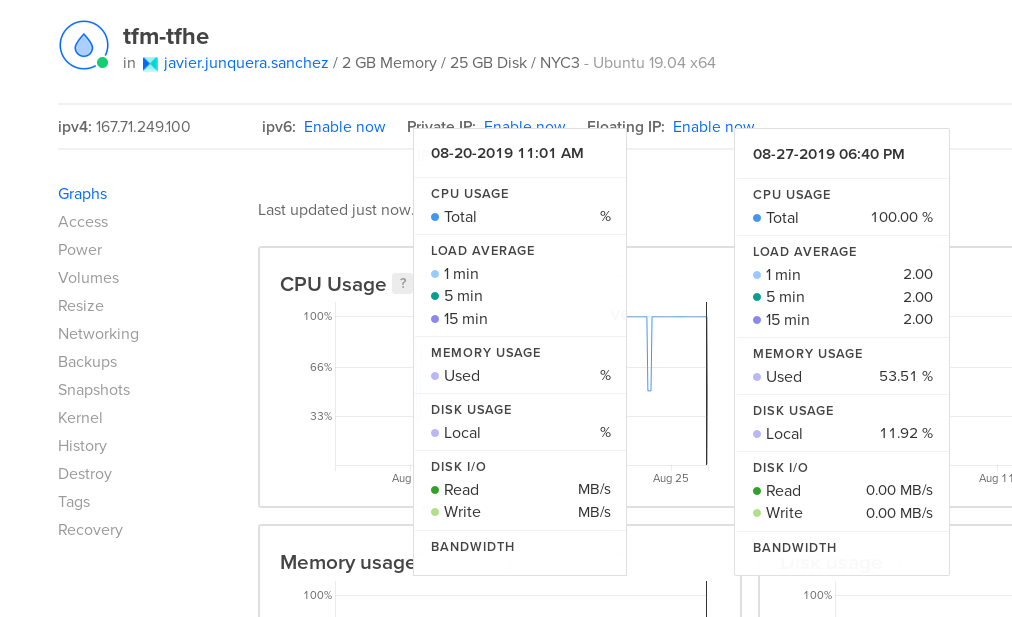
\includegraphics[width=\textwidth]{stats-do}
    \caption{Panel web de estadísticas del servidor}
    \label{fig:stats-do}
\end{figure}
